\documentclass[a4paper, 12pt]{article}

\usepackage{hyperref}
\usepackage{pgf-pie}

\hypersetup{
	colorlinks,
	linkcolor={black},
	citecolor={black},
	urlcolor={black}
}
\usepackage{lmodern}
%\usepackage{geometry}
%\usepackage{layout}
\usepackage{graphicx}
\usepackage{wrapfig}
\usepackage[OT1,T2A]{fontenc}
\usepackage[utf8]{inputenc}
\usepackage[english,bulgarian]{babel}
\usepackage{tcolorbox}
%\usepackage{lipsum}
%\tcbuselibrary{skins,breakable}
%\usetikzlibrary{shadings,shadows}
%\usepackage[framemethod=tikz]{mdframed}

\title{Виртуален асистент}
\author{Алекс Цветанов \& Антоан Георгиев}	

\newcommand{\titleGP}{\begingroup
	\centering
	%\vspace{\baselineskip}
	\rule{\textwidth}{1.6pt}\vspace{-\baselineskip}\vspace{2pt}
	\rule{\textwidth}{0.4pt}\\[\baselineskip]
	
	{\LARGE Виртуален асистент}\\[0.2\baselineskip]
	
	\rule{\textwidth}{0.4pt}\vspace{-\baselineskip}\vspace{3.2pt}
	\rule{\textwidth}{1.6pt}\\[\baselineskip]
	\begin{wrapfigure}{r}{0.35\textwidth}
		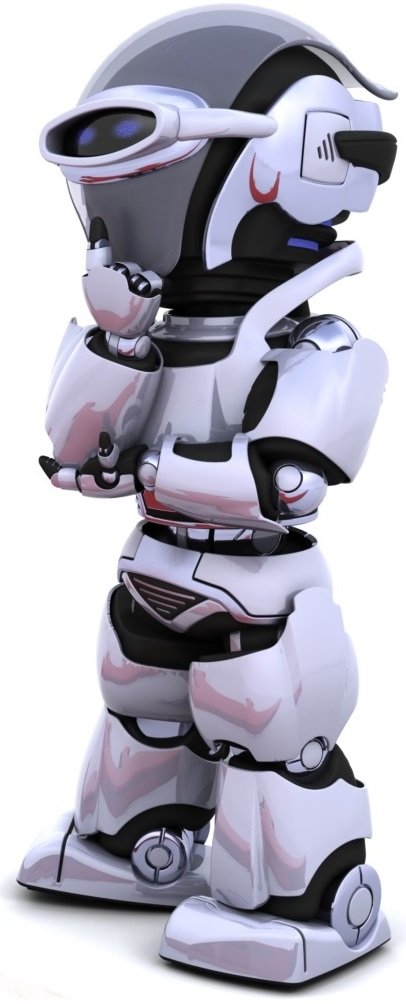
\includegraphics[scale=0.5]{../logo.png}
	\end{wrapfigure}
	
	\vspace{50pt}
	{\LARGE Алекс Цветанов\\\par}
	%{\itshape \Large Софийска Математическа Гимназия \\ София, България\par}
	{\itshape \Large София, България\par}
	{\itshape \LARGE \& \par}
	{\LARGE Антоан Георгиев\\\par}
	%{\itshape \Large ... \\ Монтана, България\par}
	{\itshape \Large Монтана, България\par}
	
	\vspace{2\baselineskip}
	
	{\scshape \large
		Под ръководството на \\
		\hspace{-0.3cm}\href{https://bg.linkedin.com/in/zlatogor-minchev-a101b85}{Доц. д-р Златогор Минчев} \\\par
	}
	\vspace{1cm}
	
	
	\vfill
	
	{\scshape Ученически иснтитут към Българска академия на науките, 2017} \\[0.3\baselineskip]
	{\large София, България }\par
	
	\endgroup}

%\mdfdefinestyle{mystyle}{%
%linecolor=green!40!black,outerlinewidth=1pt,%
%frametitlerule=true,frametitlefont=\sffamily\bfseries\color{white},%
%frametitlerulewidth=1pt,frametitlerulecolor=green!40!black,%
%frametitlebackgroundcolor=green!40!black,
%backgroundcolor=green!5,
%innertopmargin=\topskip,
%roundcorner=5pt
%}
%\newmdenv[style=mystyle]{exa}
%\newenvironment{myblock}[1]
%  {\begin{exa}[frametitle=#1]}
%  {\end{exa}}
\newenvironment{myblock}[1]
  {\begin{tcolorbox}[colback=green!5,colframe=green!40!black,title=#1]}
  {\end{tcolorbox}}

\begin{document}

	\titleGP
	\newpage
	
	\tableofcontents
	\newpage
	
	\begin{abstract}
		Изградени са много системи за управление на обучението, но нито една от тях не използва най-новите технологии в обучението (няма система, която да обединява изкуствения интелект и виртуалната реаност в едно).
		%In fact there are a lot of built-in learning management systems, but there are not any system that combines the newest technologies in education - there are not any system that uses artificial intelligence and virtual reality at once. 
		\\
		\\
		Основната цел на нашия проект е създаването на система, която да използва тези технологии и да създадем „виртуален асистент“, който да конбинира най-добрите практики в организирането на обучения, така че да са интересни, полезни и максимално улеснени за учениците. Най-важната част от проекта ни е да стимулираме учениците, показвайки им, че предметите не са толкова трудни, колкото изглеждат.
		%The core aim of our project is to create system that combines these techniques and to build "artificial teacher" that combines best practices in organizing training so that it will be interesting, useful and much easier for the students. The most important part of our project is to fertilize students, showing them that their subjects is not as difficult as sound.
		\\
		\\		
		%Teacher will train student by lessons and different types of exercises which will include theoretical part, but will mostly be oriented practically. 
		Асистентът ще помага на учениците като отговаря на въпросите им към уроците и като им дава различни по тип задачи, които ще включват теоретична част, но в по-голяма степен ще са ориентирани към практиката.
	\end{abstract}
	\vspace{1cm}
	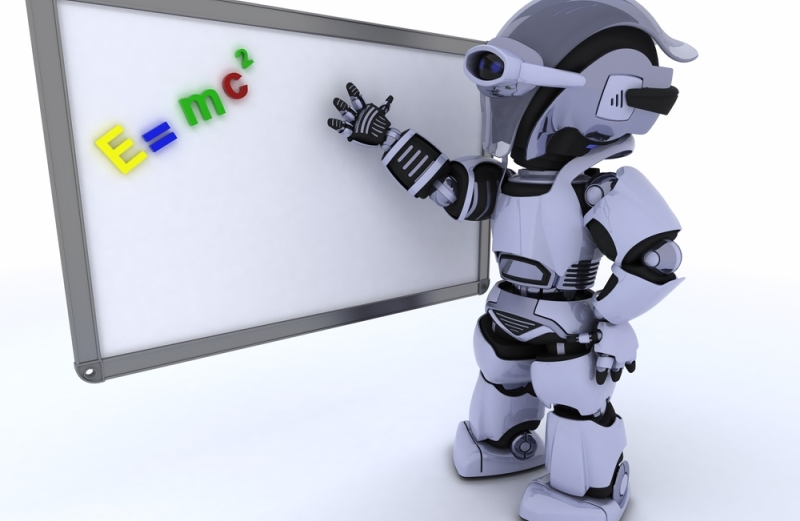
\includegraphics[width=\textwidth]{../robot-teacher.jpg}
	\newpage
	
	\section{Въведение}
	
	\vspace{1cm}
	\large{
		\begin{myblock}{"Система за управление на обучението"}
			Това е софтуер за администриране, документиране, приследяване, публикуване и получаване на обучителни курсове и тренировачни програми.
			\rule{\textwidth}{0.4pt}
			{
				\begin{flushright}
					{\Large Wikipedia}
				\end{flushright}
			}
		\end{myblock}
		\vspace{1cm}
		\begin{myblock}{"Виртуален асистент"}
			Това е система, която трябва да помага на учениците по интерактивен, интересен, полезен и по-лесен начин за тях. Тя може да бъде представена като "индивидуален ментор" по съответния предмет.
		\end{myblock}
		\vspace{1cm}
		Изградени са доста системи за управление на обучението, но все още няма такава, която да комбинира изкуствения интелект с виртуалната реалност.\\
		%There are a lot of built-in learning management systems, but there are not any system that combines artificial intelligence and virtual reality at once. \\
		\\
		Основната цел на нашия проект е създаването на „виртуален асистент“, чрез най-новите технологии и прилагайки най-добрите практики при организирането на обучения, така че да са интерактивни, интересни, полезни и възможно най-улеснени за учениците. Най-важната част от проекта ни е да стимулираме учениците, показвайки им, че предметите не са толкова трудни, колкото изглеждат. \\
		%The aim of our project is to create system that to build "artificial teacher" by following newest technologies and best practices in organizing training so that it will be interactive, interesting, useful and much easier for the students. The most important part of our project is to fertilize students, showing them that their subjects is not as difficult as sound.\\
		\\
		Асистентът ще отговаря на въпросите на учениците по съответните уроци и ще им предоставя допълнителна информация по темите, от които се интересуват.		
		%Teacher will train student by lessons and different types of exercises which will include theoretical part, but will mostly be oriented practically. 
	}
	\section{Имплементационни детайли}%Implementation
		Проектът е разделен на три части: %The project is divided into three parts:
		\begin{itemize}
			\item[Външен вид] Дизайнът имплементира мимики на лицето, за да може да намали коефициентът на нералност по време на обучението и за да подобри реалистичността на целялата комуникация. 
			%\item[appearance] Design, which must implement human facial expressions for better and realistic interactive communication. 
			\item[интелект] Приложно-програменият интерфейс ще отговаря на въпросите на учениците и ще връща полезната за тяхната сфера на развитие информация \\ \\ Той използва текст/урок на базата, на който отговаря на въпроси, също така ще използва база данни, генерирана от представителни сайтове с коректа информация по съответните теми.
			%\item[intelligence] Application Programming Interface that must return material which must be learnt by student \\ \\ This interface uses data base to make information which will be used to build knowledge base where data base is simple data about how students visit resources and knowledge base is system of logical conditions.
			\item[комуникация] За осъществяване на комуникацията се използват инструменти, превръщащи говорът в текст, който текст бива „разбран“ от асистента 
			%\item[communication] Live bot chat for all questions during the lesson that "artificial teacher" presents. 
		\end{itemize}
		{\centering
			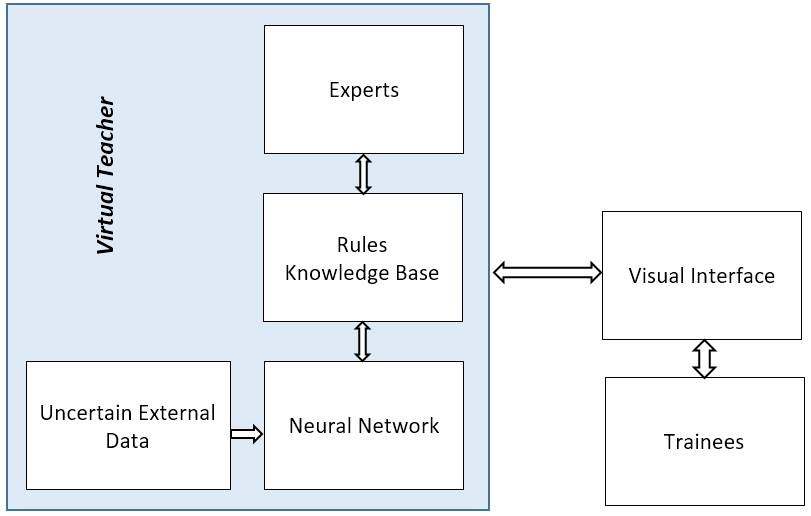
\includegraphics[width=\textwidth]{../schema.jpg}
		}
		Всяка част има свойте специфики, което прави проектът още по-предизвикателен, но в крайна сметка целта е да предоставим едно различно обучение с модерен поглед към бъдещето.
		%Each part has a lot of specifics and the project is quite challenging, but it would give a different, modern outlook to the future learning process.
		\subsection{Проблеми}
			\subsubsection{Приложно-програмен интерфейс}
			    Процесът по анализиране на текст не е толкова голям проблем, зареди вече готовите инстументи за езика Python. По-големият проблем е с „разбирането“ на самия текст и изграждането на мрежа от думи, така че тя да представя случващото се в изречението/текста действие или случка. \\ \\
			    За втората част няма изработени стабилни библиотеки и модули, което ни накара да си ги пишем сами, което се оказа не лесна задача, поради което все още не е напълно работещо „разбирането на текст“.
			\subsubsection{Дезайн}
			    АНТОАН ГЕОРГИЕВ ДА СЕ ЗАЕМЕ
			\subsubsection{Communication}
				АНТОАН ГЕОРГИЕВ ДА СЕ ЗАЕМЕ
	\section{Технологии и инструменти}
	\begin{itemize}
		\item Python \& NLTK модул в комбинация с анализатора на текст от Станфордския университет
		\item АНТОАН ГЕОРГИЕВ ДА СЕ ЗАЕМЕ
	\end{itemize}
	\newpage
	\section{Бъдещо развитие}
	\begin{wrapfigure}{l}{0.35\textwidth}
		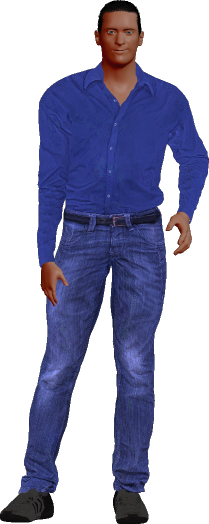
\includegraphics[scale=0.35]{../bad_boy.png}
	\end{wrapfigure}
	Бъдещото развитие на проекта включва добавяне на мимики на лицето на 3D моделът ни съвместно с психолози, както и подобряване на „интелекта“ на асистента и прилагането на технологиятав училищата, започвайки от Софийската професионална гимназия по електроника „Джон Атанасов“ и Софийската математическа гимназия „Паисий Хилендарски“. \\ \vspace{0.5cm}
	\begin{center}
		\begin{myblock}{Въпроси от анкета}
			\begin{enumerate}
				\item Подкрепяте ли изграждането на онлайн система за обучение и прилагането ѝ в училище?
			\end{enumerate}
		\end{myblock}
	\end{center}
	The diagram shows the results of non-representative survey conducted among 55 students of SHSM: \\
	\begin{center}
		\begin{tikzpicture}
			\pie[cloud, text=inside, scale font]{95/Yes, 3/No, 2/}
		\end{tikzpicture}
	\end{center}

	So those results stimulate us to make it better and better and to make it make more interesting, more interactive and more entertaining.
%	\newpage
 	\section{Acknowledgments}
 	 	 Special thanks to:
 	 	 \begin{itemize}
 	 	 	\item Zlatogor Minchev for the improvement of the idea
 	 	 	\item Emil Kelevejiev for the improvement of the documentation
 	 	 \end{itemize}
 	 	 Thanks also to:
 	 	 \begin{itemize}
 	 	 	\item High School Students Institute of Mathematics and Informatics
 	 	 	\item Bulgarian Academy of Sciences
 	 	 	\item Sofia High School of Mathematics
 	 	 \end{itemize}
 	 	 \begin{thebibliography}{99}
 	 	 	\bibitem{book1}
 	 	 	{\itshape Artificial Intelligence: A Modern Approach, \\ 3rd Edition, Prentice Hall, 2010}. \\
 	 	 	\texttt{Stuart Russell \& Peter Norvig.} \\
  	 	    \bibitem{virtobjects}
   	        {\itshape Virtual\ objects\ seem\ totally\ real}.
            \texttt{https://www.theverge.com/2017/8/1/16070188/\\
            avegant-light-field-display-ar-headset-next-level-video}. \\
 	 	 	\bibitem{Amelia}
 	 	 	{\itshape Amelia}.
 	 	 	\texttt{http://www.ipsoft.com/amelia/}. \\
 	 	 	\bibitem{The Future Of Chatbots And Artificial Intelligence}
 	 	 	{\itshape The Future Of Chatbots And Artificial Intelligence}.
 	 	 	\texttt{https://www.lifehacker.com.au/2016/05/meet-viv-the-future\\
 	 	 		-of-chatbots-and-artificial-intelligence/}. \\
 	 	 	
 	 	 	\bibitem{Your DNA Avatar – What Happens When Artificial Intelligence Meets Cutting-Edge Genetics?}
 	 	 	{\itshape Your DNA Avatar - What Happens When Artificial Intelligence Meets Cutting-Edge Genetics?}.
 	 	 	\texttt{https://www.wilsoncenter.org/blog-post/your-dna-avatar-\\
 	 	 		    what-happens-when-artificial-intelligence-meets-cutting-\\
 	 	 		    edge-genetics}. \\
 	 	 	
 	 	 	\bibitem{mariadbpp}
 	 	 	{\itshape MariaDB++}.
 	 	 	\texttt{https://mariadb.org/}. \\
 	 	 	\bibitem{gcc}
 	 	 	{\itshape GNU Compiler Collection}.
 	 	 	\texttt{https://gcc.gnu.org/}. \\
 	 	 	Copyright \copyright\  2009 Free Software Foundation, Inc.
 	 	 	\bibitem{mariadb}
 	 	 	{\itshape MariaDB}.
 	 	 	\texttt{https://mariadb.org/}. \\
 	 	 	Copyright \copyright\  2017 MariaDB Foundation
 	 	 	\bibitem{mariadb}
 	 	 	{\itshape MariaDB++}.
 	 	 	\texttt{https://mariadb.org/}. \\
 	 	 	Copyright \copyright\  2017 MariaDB Foundation
 	 	 	\bibitem{latex}
 	 	 	{\itshape \LaTeX}.
 	 	 	\texttt{https://www.latex-project.org/}.
 	 	 \end{thebibliography}
\end{document}
